\subsection{Двустороннее затухание}

Рассмотрим семейство функций 
\begin{equation}
    f(t) = ae^{-b|t|}
    \label{eq:fade_function}
\end{equation}

\subsubsection{Графики исходных функций}

Графики данной функции при различных значениях $a$ и $b$ представлены на рисунках \ref{fig:fade_1}, \ref{fig:fade_2} и \ref{fig:fade_3}.
\begin{figure}[ht!]
    \centering
    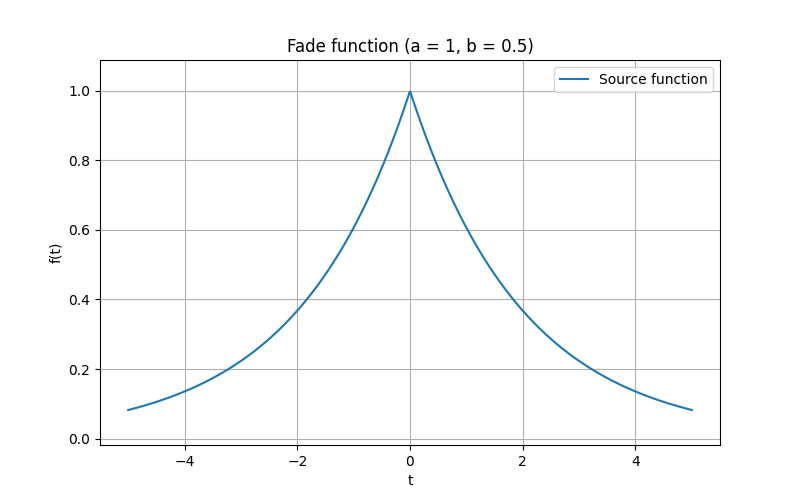
\includegraphics[width=\textwidth]{media/fade_1.png}
    \caption{График функции $f(t)$ при $a = 1$, $b = 0.5$}
    \label{fig:fade_1}
\end{figure}

\begin{figure}[ht!]
    \centering
    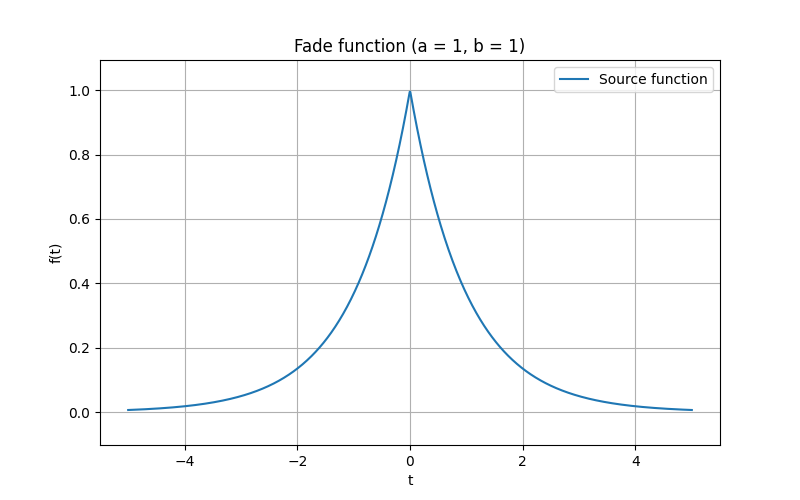
\includegraphics[width=\textwidth]{media/fade_2.png}
    \caption{График функции $f(t)$ при $a = 1$, $b = 1$}
    \label{fig:fade_2}
\end{figure}

\begin{figure}[ht!]
    \centering
    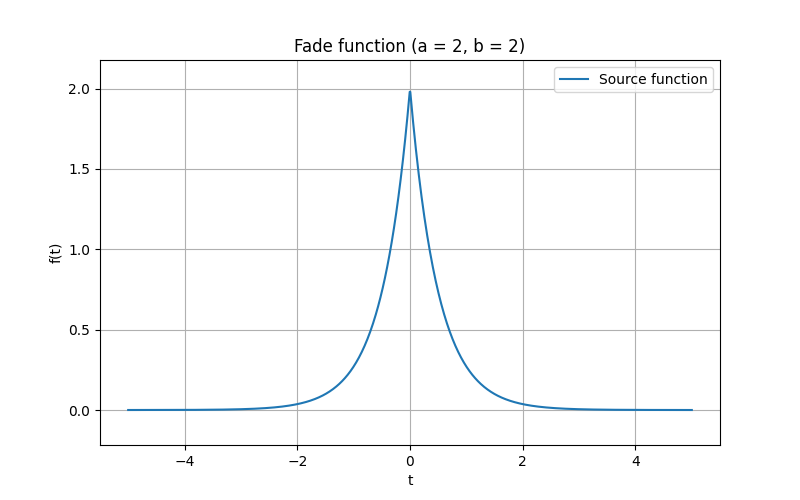
\includegraphics[width=\textwidth]{media/fade_3.png}
    \caption{График функции $f(t)$ при $a = 2$, $b = 2$}
    \label{fig:fade_3}
\end{figure}

\subsubsection{Нахождение образа функции}
Согласно формуле \eqref{eq:image_from_function}, Фурье образ функции $f(t)$ задается следующим выражением:
\begin{multline}
    \hat{f}(\omega) = \frac{1}{\sqrt{2\pi}} \int_{-\infty}^{\infty} f(t) e^{-i\omega t} dt = \frac{1}{\sqrt{2\pi}} \left(\int_{-\infty}^{0} ae^{bt} e^{-i\omega t} dt + \int_{0}^{\infty} ae^{-bt} e^{-i\omega t} dt\right) = \\
    \frac{a}{\sqrt{2\pi}} \left(\int_{-\infty}^0 e^{t(b -i \omega)}dt + \int_0^{\infty} e^{t(-b - i\omega)}dt\right) = \frac{a}{\sqrt{2 \pi}} \left( \frac{1}{b - i\omega} + \frac{1}{b + i\omega}\right) = \frac{\sqrt{2/\pi}ab}{b^2 + \omega^2}
    \label{eq:fade_function_image}
\end{multline}

\subsubsection{Графики образов функций}
Графики образов функции при различных значениях $a$ и $b$ представлены на рисунках \ref{fig:fade_1_image}, \ref{fig:fade_2_image} и \ref{fig:fade_3_image}.

\begin{figure}[ht!]
    \centering
    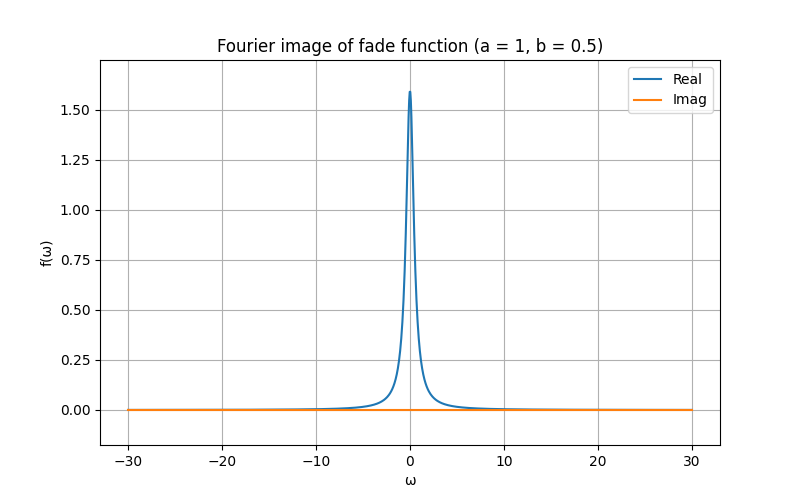
\includegraphics[width=\textwidth]{media/fade_1_image.png}
    \caption{График образа функции $f(t)$ при $a = 1$, $b = 0.5$}
    \label{fig:fade_1_image}
\end{figure}

\begin{figure}[ht!]
    \centering
    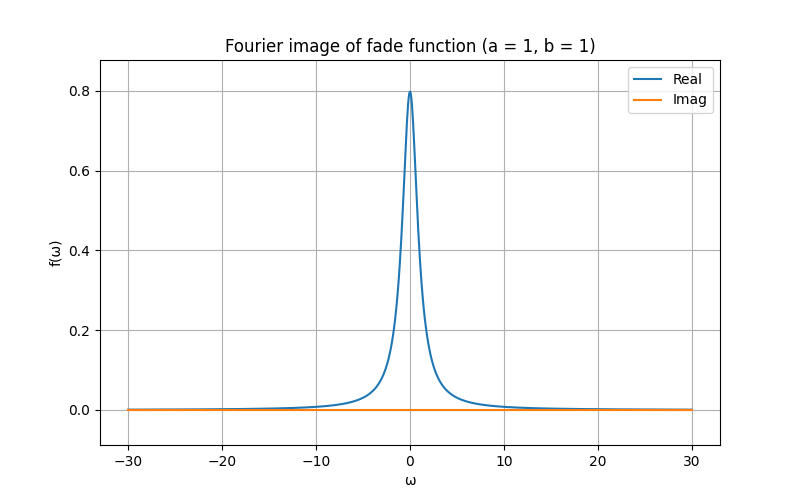
\includegraphics[width=\textwidth]{media/fade_2_image.png}
    \caption{График образа функции $f(t)$ при $a = 1$, $b = 1$}
    \label{fig:fade_2_image}
\end{figure}

\begin{figure}[ht!]
    \centering
    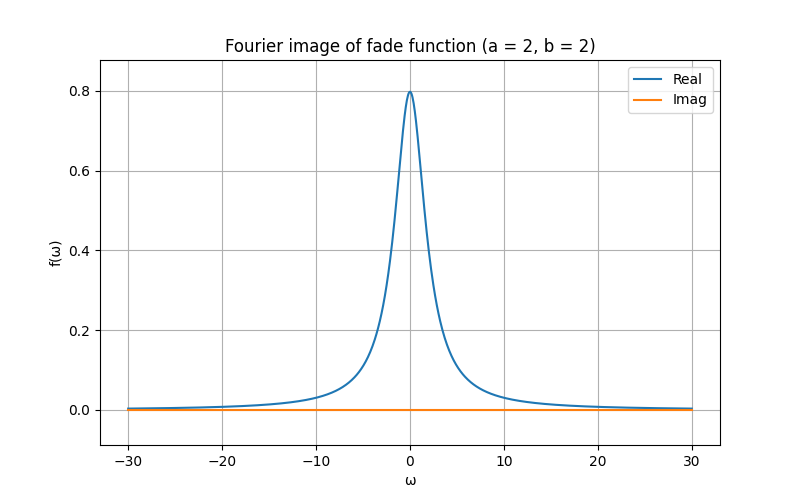
\includegraphics[width=\textwidth]{media/fade_3_image.png}
    \caption{График образа функции $f(t)$ при $a = 2$, $b = 2$}
    \label{fig:fade_3_image}
\end{figure}

\FloatBarrier
\subsubsection{Проверка равенства Парсеваля}
Проверим равенство Парсеваля (см. формулу~\eqref{eq:parseval_indentity}). Для этого воспользуемся функцией \texttt{parseval\_check}.
% table with parseval check results
\begin{table}[ht!]
    \centering
    \begin{tabular}{|c|c|}
        \hline
        $\displaystyle\int_{-100}^{100}{|f(t)|^2}$ & $\displaystyle\int_{-100}^{100}{|\hat{f_1}(\omega)|^2}$ \\
        \hline
        1.9998 & 1.9998 \\
        \hline
    \end{tabular}
    \caption{Результаты проверки равенства Парсеваля для функции затухания $f(t)$ при $a = 1$, $b = 0.5$}
    \label{tab:fade_1_parseval_check}
\end{table}

\begin{table}[ht!]
    \centering
    \begin{tabular}{|c|c|}
        \hline
        $\displaystyle\int_{-100}^{100}{|f(t)|^2}$ & $\displaystyle\int_{-100}^{100}{|\hat{f_2}(\omega)|^2}$ \\
        \hline
        0.9997 & 0.9997 \\
        \hline
    \end{tabular}
    \caption{Результаты проверки равенства Парсеваля для функции затухания $f(t)$ при $a = 1$, $b = 1$}
    \label{tab:fade_2_parseval_check}
\end{table}

\begin{table}[ht!]
    \centering
    \begin{tabular}{|c|c|}
        \hline
        $\displaystyle\int_{-100}^{100}{|f(t)|^2}$ & $\displaystyle\int_{-100}^{100}{|\hat{f_3}(\omega)|^2}$ \\
        \hline
        1.9978 & 1.9978 \\
        \hline
    \end{tabular}
    \caption{Результаты проверки равенства Парсеваля для функции затухания $f(t)$ при $a = 2$, $b = 2$}
    \label{tab:fade3_parseval_check}
\end{table}

Видим, что во всех случаях значения почти не отличаются друг от друга. Различие, по большей части, обусловлено тем, что в программе нельзя найти интеграл по бесконечности, поэтому просто берется достаточно большой интервал интегрирования.

\subsubsection{Анализ результатов}
Влияние параметров $a$ и $b$ на графики функции и ее образа можно описать следующим образом, в соответствиями с формулами \eqref{eq:fade_function} и \eqref{eq:fade_function_image}: $a$ отвечает за амплитуду функции, а $b$ за скорость затухания. При увеличении $a$ амплитуда функции увеличивается, а при увеличении $b$ функция затухает быстрее. 
